\section{Le 6W}\label{6w}

Il problema principale degli utenti è il \textit{tempo}: ciò fa riflettere su come comunicare l'informazione nel migliore dei modi, tema già affrontato nel giornalismo.
La miglior organizzazione dell'informazione si ha quando vengono seguiti i 6 assi informativi principali, ovvero le \textit{6W}: \textit{Who}, \textit{What}, \textit{Why}, \textit{Where}, \textit{When}, \textit{How}.\\
Alcuni assi però sono più importanti di altri:
\begin{itemize}[noitemsep]
	\item Obbligatori: \textit{Who}, \textit{What}, \textit{Where}
	\item Opzionali: \textit{When}
	\item Opzionali consigliati: \textit{Why}, \textit{How}
\end{itemize}
\par Un sito ben progettato che segue queste regole deve essere in grado di poter fornire all'utente l'informazione che cerca e gli strumenti per continuare a navigare chiaramente al suo interno, facendo che già dopo un click sia convinto a restare nella piattaforma.
\par Bisogna sempre tenere conto che gli utenti hanno \textit{alte aspettative} e \textit{secondi contati}.
\par In questa sezione vengono quindi analizzati tali assi per quanto riguarda la homepage del sito e una pagina che rappresenta un evento, entrambi documenti allegati a questo documento, come descritto in Sez.~\ref{allegati}.

\subsection{Who?}
	\begin{quote}
	    \emph{``Chi rappresenta il sito?''}
	\end{quote}
	La risposta a questa prima domanda è data principalmente dal \textit{logo} del sito.
	\par In questo caso particolare, il logo (Fig.~\ref{fig:logo}) è presente su ciascuna pagina interna del sito in alto a sinistra (uno dei primi punti in cui l'utente focalizza lo sguardo), in quanto l'header (Fig.~\ref{header}) viene ripetuto in maniera uguale su tutte le pagine.
	\par Il logo, \textit{ticketone.it}, è scritto in caratteri minuscoli con un font facilmente comprensibile.
	Al suo interno è presente anche il dominio, questo aiuta l'utente a ricordarlo interamente in maniera più facile.
	I colori sono bianco e giallo, piacevolmente in contrasto con il blu dello sfondo.
	\par Questa considerazione vale sia per la homepage di TicketOne che per qualsiasi altra pagina contenuta al suo interno.
	
\subsection{Where?}
	\begin{quote}
		\emph{``A che tipo di sito sono arrivato? Come sono posizionato all'interno della gerarchia?''}
	\end{quote}
	Il \textit{where} è uno degli assi informativi più importanti in quanto permette all'utente di sapere dove si trova all'interno del sito.
	Questo può venire implementato in vari modi da parte degli sviluppatori:
	\begin{itemize}[noitemsep]
		\item \textit{location} con l'uso di \textit{breadcrumb};
		\item \textit{attribute} utilizzando tag per dividere le pagine in categorie;
		\item \textit{path} dinamici che mostrano all'utente le pagine già visitate.
	\end{itemize}
	
	\paragraph{Homepage}
		L'hompage rende abbastanza evidente la sua posizione come pagina di benvenuto al sito, dalla quale si può navigare tra categorie, eventi specifici, località, oppure effettuare ricerche più approfondite (Sez.~\ref{ricerca}).

	\paragraph{Pagina evento}
		All'interno della pagina di ciascun evento è possibile notare che, a fianco del logo e sotto allo slogan, è presente il nome dell'evento (Fig.~\ref{where}).
		
		\begin{figure}[hbt]
			\centering
			
\includegraphics[width=10cm]{img/where.png}
			\caption{Nome dell'evento a fianco al logo}
			\label{where}
		\end{figure}
	
		Oltre a questo, è possibile capire a che evento la pagina si sta riferendo in quanto al centro della pagina si può trovare un fac simile del biglietto relativo a tale evento (Fig.~\ref{where2}).
		\begin{figure}[hbt]
			\centering
			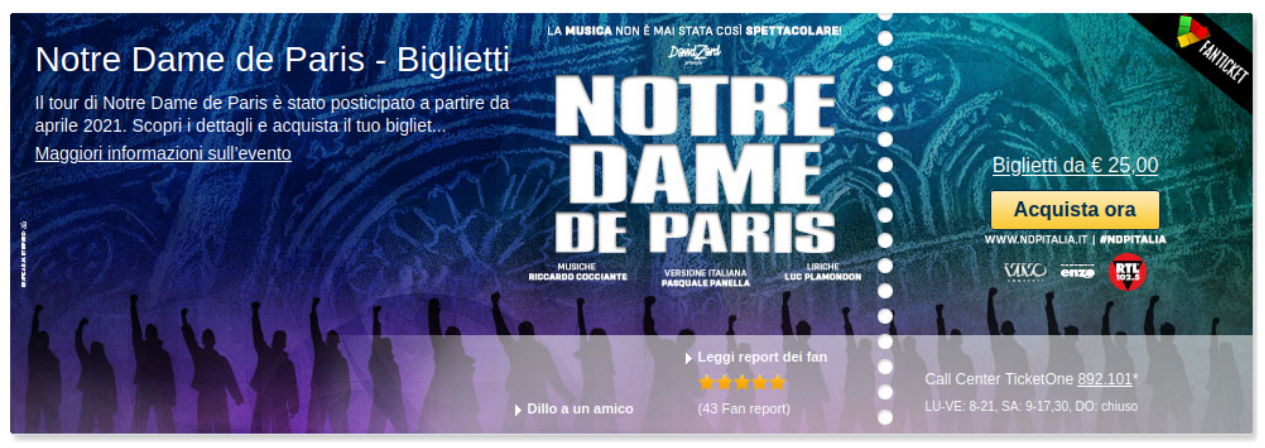
\includegraphics[width=\textwidth]{img/where2.png}
			\caption{Fac simile biglietto}
			\label{where2}
		\end{figure}
	
\subsection{What?}
	\begin{quote}
		\emph{``Cosa offre il sito?''}
	\end{quote}
	\paragraph{Homepage}
		L'homepage del sito dice chiaramente cosa TicketOne offre ai suoi utenti: la possibilità di comprare biglietti a eventi musicali, sportivi, ecc. su tutto il territorio italiano e non solo.
		Questo si capisce principalmente dal carosello degli eventi presentato in primo piano all'utente e successivamente dal menu laterale che permette di navigare per le principali categorie di eventi oppure per le maggiori città italiane.
		
	\paragraph{Pagina evento}
		La pagina di evento risponde facilmente a cosa offre in quanto, oltre al fac simile del biglietto (Fig.~\ref{where2}), è presente la lista dei biglietti disponibili.
		\begin{figure}[hbt]
			\centering
			\includegraphics[width=\textwidth]{img/what.png}
			\caption{Lista biglietti disponibili per evento}
			\label{what}
		\end{figure}
	
\subsection{When?}
	\begin{quote}
		\emph{``Quali sono le ultime novità? Quando è stato mantenuto per l'ultima volta?''}
	\end{quote}
	\paragraph{Homepage}
		A questa domanda risponde facilmente la homepage del sito in quanto le ultime novità vengono mostrate all'utente tramite il carosello degli eventi in evidenza (Fig.~\ref{homepage}).
		Chi entra nel sito è in grado di individuare velocemente gli eventi programmati per i mesi successivi.
	\paragraph{Pagina evento}
		Nelle pagine dell'evento è possibile trovare gli aggiornamenti relativi o i cambiamenti a date specifiche all'interno di un box giallo, posizionato sotto al fac simile del biglietto e sopra alla lista dei biglietti disponibili.
		\begin{figure}[hbt]
			\centering
			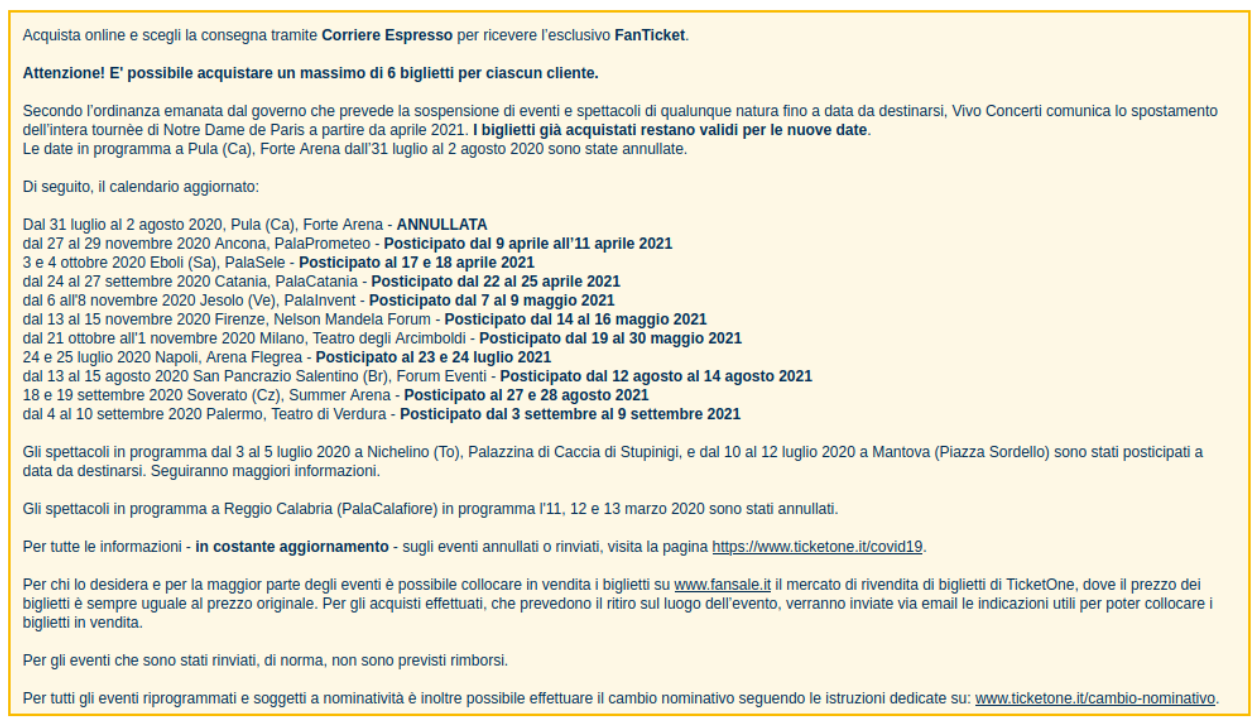
\includegraphics[width=\textwidth]{img/when.png}
			\caption{Box di aggiornamenti riguardo della pagina eventi}
			\label{when}
		\end{figure}
		
\subsection{Why?}
	\begin{quote}
		\emph{``Perchè mai dovrei fermarmi su questo sito? Quali benefici mi porta?''}
	\end{quote}
	La domanda a questa risposta viene data di solito dallo \textit{slogan}.
	Per TicketOne questo è ``\textit{Biglietti, Concerti, Spettacolo, Sport \& Cultura}'' e viene specificato alla destra del logo, nel header di ciascuna pagina.
	L'utente riesce a capire velocemente di cosa si tratta e cosa il sito offre.
	\par La risposta a questa domanda vale sia per la homapage del sito che per le altre pagine come quella evento in allegato.
		
\subsection{How?}
	\begin{quote}
		\emph{``Come faccio ad arrivare alle sezioni principali?''}
	\end{quote}
	\paragraph{Homepage}
		Il \textit{how} si riverisce a come l'utente può ricercare le informazioni e quindi navigare all'interno del sito in maniera intuibile.\\
		La ricerca, come spiegato in Sez.~\ref{ricerca} parte dalla barra posta all'interno del header.
		L'utente, avendo a disposizione i suggerimenti di ricerca, riesce facilmente a capire come vengono distribuiti gli eventi (per categorie, per artista, per località, ecc.) e come navigare TicketOne.
		\par Nello specifico, l'homepage presenta sulla sinistra del carosello degli eventi principali un menu che permette all'utente di visualizzare velocemente gli eventi divisi per categorie principali e per località maggiori.
		
	\paragraph{Pagina evento}
		Per quanto riguarda la pagina riferita ad un evento, rimane possibile la ricerca tramite la barra presente nell'header.
		